\documentclass[10pt]{article}
\usepackage[letterpaper,margin=1in]{geometry}
\usepackage[T1]{fontenc}
\usepackage{newtxtext,newtxmath}
\usepackage{graphicx}
\usepackage{booktabs}
\usepackage{amsmath}
\usepackage{xcolor}
\usepackage[numbers,sort&compress]{natbib}
\usepackage{caption}
\usepackage{enumitem}
\usepackage{tikz}
\usetikzlibrary{arrows.meta,positioning,fit,shapes.geometric}
\usepackage[colorlinks=true,linkcolor=blue!50!black,citecolor=blue!50!black,urlcolor=blue!50!black]{hyperref}
\usepackage{eurosym}

\captionsetup{font=small,labelfont=bf}
\setlist{nosep,leftmargin=1.4em}
\newcommand{\dream}{Dream-1}
\newcommand{\mean}[1]{\overline{#1}}

\title{\textbf{Supervising a Generalist Robot Policy Through a Rule-Bound,\\Long-Horizon Relay: A Harness, Two Simulators, and\\What the Teleoperation Data Got Wrong}}

% TODO(authors): complete surnames and affiliations before submission.
\author{
  Darsh Patel\thanks{Corresponding author. Code: \url{https://github.com/darshp848/hill-climb-harness},
  \url{https://github.com/darshp848/task_simulation}, \url{https://github.com/darshp848/follower_code}.}
  \and Kaushik
  \and Muhammad Mukthar
}
\date{Physical AI Hacks (MakerMods $\times$ Dream Labs), 7--8 November 2026\\[2pt] \small Preprint, 9 November 2026}

\begin{document}
\maketitle

\begin{abstract}
We report the system we built over a 36-hour hackathon to run a generalist vision--language--action
(VLA) policy, Dream Labs' \dream{}, through a timed three-stage relay on two brakeless 7-motor
MakerMods Metal arms: unplug USB cables from a hub, stack a tower above 4\,in, and drop legal golf
balls into a bin while avoiding an illegal ball. The rubric turns ordinary failures into match losses:
touching a later stage's object before the current pass bar is a disqualification (DQ), and binning the
illegal ball loses the match. The policy is a black box behind an HTTP station agent, so our only
inputs are discrete: which prompt to send, and when to stop, home or retry. We contribute (i) a
supervisory harness that treats the relay as a stage state machine with two-look verification, a
10\,Hz local illegal-ball guard, sensor overrides and template-only prompting, together with a
formal decision model for tuning it; (ii) two simulators, a virtual-clock stress simulator that plays
37 scenarios whose faults reuse the error types logged on the station, and a MuJoCo table driven by the real
\dream{} API with a ground-truth referee; (iii) a teleoperation pipeline for the Metal arms (a
gravity-compensated leader/follower and a Quest headset path with a wrist-flip guard); and (iv) a
diagnosis of why our fine-tune failed. Measured on the station, the median policy round trip was
1.12\,s and 67\% of 1{,}650 action chunks ran in stop-and-wait mode, leaving the arms idle about 30\%
of the time. In 185 simulated matches per configuration, a faster judge raised mean points from 61.2
to 70.5 but lost 28 matches to the illegal ball; adding the local guard kept 69.8 points and lost none.
With the real policy in MuJoCo, base \dream{} unplugged a cable in 14 of 25 matches but completed 0 of
54 put-downs. The fine-tune was worse than the base model on every task; its Quest demonstrations carried
a 5.5\,cm gravity-sag offset between commanded and measured tool pose that the leader-arm data did not.
We have no logged per-stage success rates from the physical station, and we say so wherever it matters.
\end{abstract}

\section{Introduction}

Generalist VLA policies~\cite{brohan2023rt2,kim2024openvla,black2024pi0} take a camera stream and a
sentence and return a chunk of actions. They are increasingly offered as a service: the team holds an API
key, a station agent on the robot computer runs the control loop, and the model runs elsewhere. This
changes what a team can engineer. Within a hackathon you cannot retrain the base model or add a
controller underneath it. You can choose the words, decide when a subtask is finished, stop the arms,
and collect demonstrations for a fine-tune.

The Physical AI Hacks ``Hill Climb'' relay made those choices consequential. Each team got a station with
two MakerMods Metal arms (seven Damiao motors each, no brakes), an overhead camera, one wrist camera
per arm, and \dream{} through Dream Labs' SDK. A match lasts 5 minutes, and nobody may touch the robot or
send input to the policy after ``go''. Table~\ref{tab:rubric} gives the scoring. Two rules make it unlike a
benchmark success rate. First, the stages are gated: a gripper that touches a block before a cable is out
is a DQ, and so is touching a ball before the tower stands. Second, two black (on our table, white) balls
lie among the legal ones, and binning either loses the match. A harness that declares ``done'' too early,
or one that lets the policy wander, scores zero.

This paper describes what we built and what we measured, in the order the work happened:
\begin{itemize}
  \item \textbf{A supervisory harness} (Section~\ref{sec:harness}) that never commands a motor. It runs the
  relay as a state machine over \dream{}, verifies each stage with two agreeing looks from a vision-language
  judge plus gripper sensors, guards the illegal ball with a local detector at 10\,Hz, and composes every
  prompt from tested templates. We also write its decision rules as a small set of equations so they can
  be tuned in simulation rather than by hand (Section~\ref{sec:decision}).
  \item \textbf{Measurements of the serving loop} (Section~\ref{sec:latency}): where the 1.1\,s round trip
  goes and why the arms stand still for about a third of each run.
  \item \textbf{Two simulators} (Section~\ref{sec:sims}) and the results from 185-match sweeps, a
  30-configuration judge benchmark, and 25 MuJoCo matches with the real policy (Section~\ref{sec:results}).
  \item \textbf{Teleoperation and fine-tuning} on the Metal arms (Section~\ref{sec:teleop}), including a
  diagnosis of the fine-tune's failure that traces it to the data-collection path rather than the model.
\end{itemize}
Section~\ref{sec:limits} lists what we could not measure. The main gap is plain: the station logged
policy calls but not task outcomes, so we report no physical success rate for any stage.

\begin{table}[t]
\centering
\small
\caption{Rubric v4 of the 1v1 Hill Climb Relay (abridged). Pass bars gate the next stage.}
\label{tab:rubric}
\begin{tabular}{@{}p{0.2\linewidth}p{0.34\linewidth}p{0.4\linewidth}@{}}
\toprule
Stage & Pass bar & Points \\
\midrule
1. Unplug USB cables & $\geq 1$ cable out of the hub & $+10$ first, $+5$ each further; $+20$ per loose cable plugged in (max 4) \\
2. Stack & tower $>4$\,in, free-standing 3\,s after release & $+20$; $+3$ per full inch; $+10$ taller tower (head-to-head) \\
3. Balls & none & $+5$ per legal ball in bin; illegal ball in bin $=$ match lost \\
Integrations & shown to referee before the match & $+10$ LiveKit, $+5$ Dimensional \\
\midrule
\multicolumn{3}{@{}l}{DQ: touching a later stage's object before the current pass bar; any human input after ``go''.}\\
\bottomrule
\end{tabular}
\end{table}

\section{Related work}

\paragraph{Language-conditioned policies and supervisors.}
SayCan~\cite{ahn2022saycan} and Inner Monologue~\cite{huang2022inner} put a language model above a library
of skills and feed scene feedback back into the plan; Code as Policies~\cite{liang2023code} writes the
supervisor as code. Our setting is narrower and stricter. There is one skill, a monolithic bimanual VLA, and
the interface is a single prompt for both arms. The supervisor must also respect gating rules whose
violation is not recoverable.

\paragraph{Success detection.} Using vision-language models to judge task success has been studied
directly~\cite{du2023success}, and REFLECT~\cite{liu2023reflect} uses them to explain failures. We use a
judge for both stage completion and a safety guard, and we find that the guard question is the harder one
for most models (Section~\ref{sec:judges}).

\paragraph{Teleoperation and data.} Leader/follower arms~\cite{zhao2023aloha,wu2023gello} and LeRobot
datasets~\cite{cadene2024lerobot} are now the default path to fine-tuning data. Our diagnosis in
Section~\ref{sec:ft} is a case where two collection paths on the same arm produced inconsistent
state-to-action maps, which the loss curve did not reveal.

\paragraph{Evaluation in simulation.} SIMPLER~\cite{li2024simpler} warns that simulated evaluation is
useful only when the simulator's noise matches reality. We report the stress simulator's numbers as tests of
harness logic only, and we keep them apart from the MuJoCo runs with the real policy. For uncertainty we
follow the bootstrap reporting advocated by Agarwal et al.~\cite{agarwal2021precipice}.

\section{Platform}
\label{sec:platform}

\begin{figure}[t]
\centering
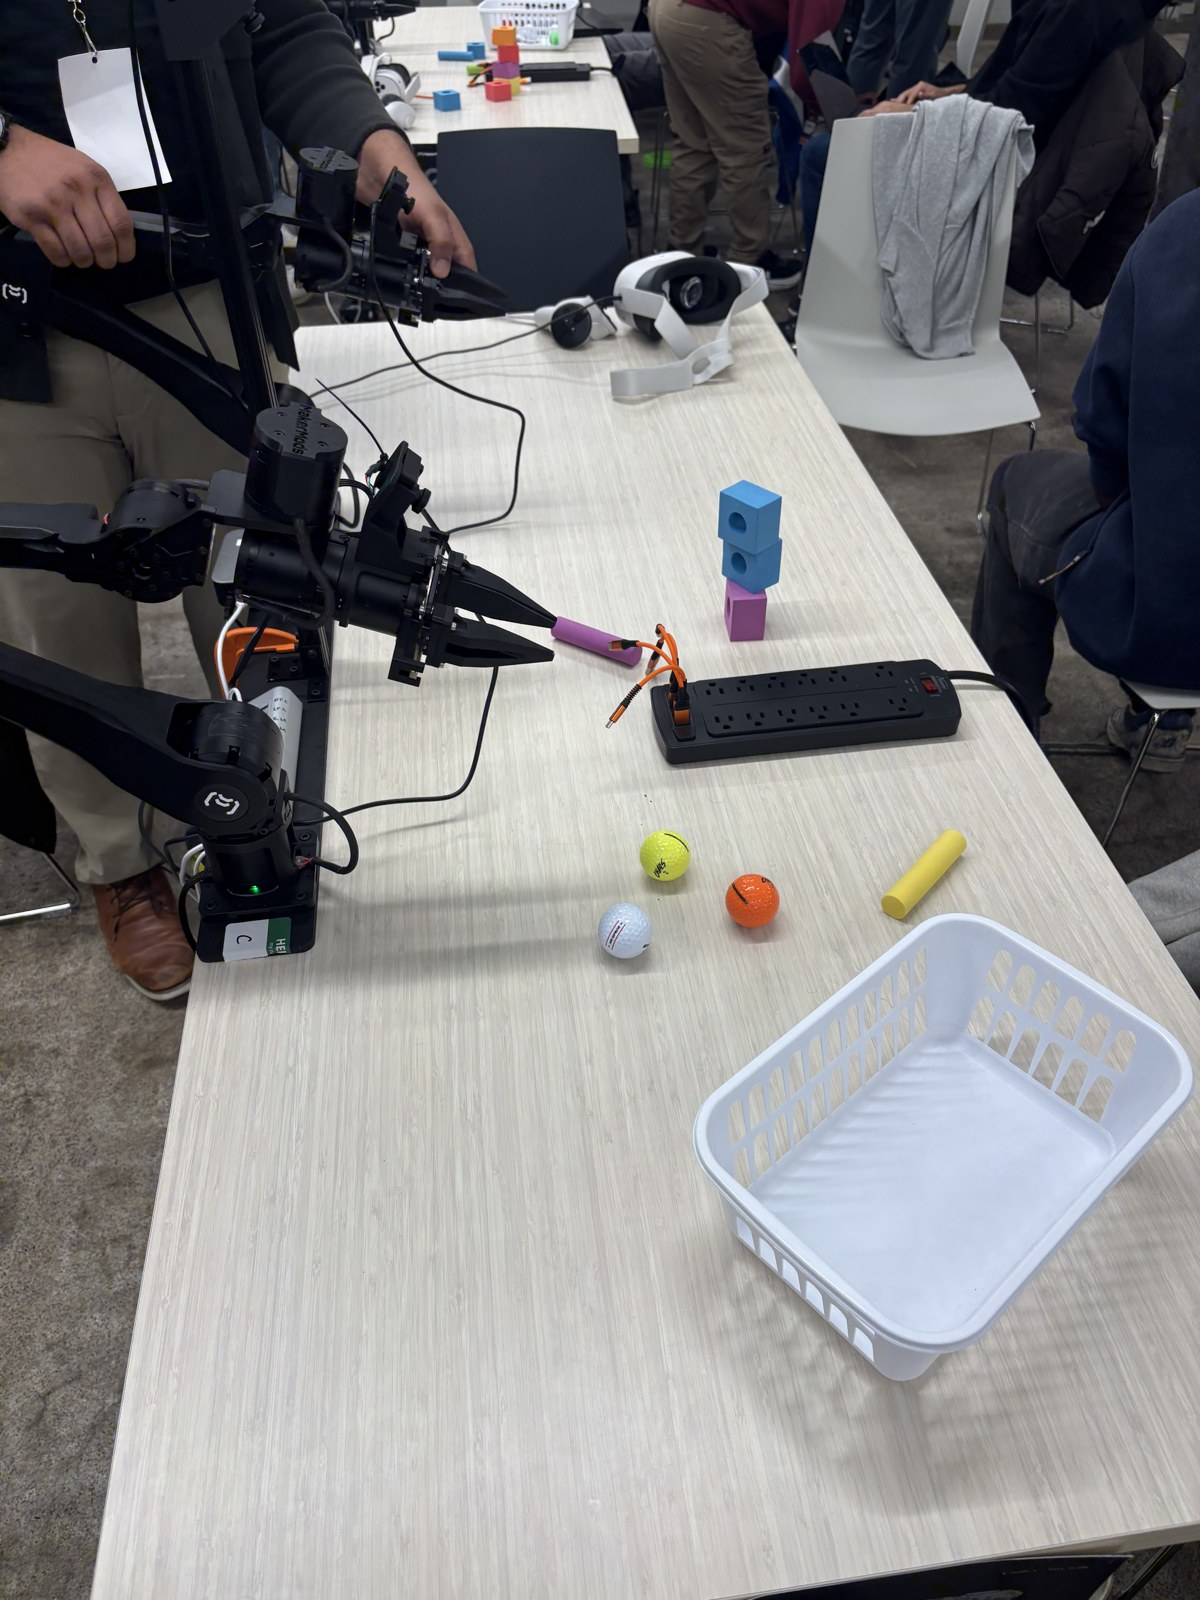
\includegraphics[width=0.36\linewidth]{../docs/station_c_setup.jpg}
\caption{Station C on 7 November. Two MakerMods Metal arms on a rail, the overhead camera on the
centre pole, and a wrist camera on each gripper. On the table: the power strip with orange USB cables
(stage 1, unplugged from the wall), blue and pink foam cubes and yellow/pink sticks (stage 2), golf balls and
the white bin (stage 3). On this table the white golf ball is the illegal one.}
\label{fig:station}
\end{figure}

\paragraph{Hardware.} Figure~\ref{fig:station} shows the station. Each Metal arm has six joints plus a
gripper, driven by Damiao motors over CAN at 1\,Mbit/s from an Intel NUC. The station agent declares
\texttt{body: metal}. Early on, an installed YAM driver library misled us into treating the arms as YAM arms;
our leader/follower code now refuses to run unless the station config names the arm type it was written for.

\paragraph{Control stack.} We read the station's installed SDK (\texttt{dreamlabs} 1.0.37). The policy returns
48-row chunks, played at a policy rate of 20\,Hz (2.4\,s per chunk). A command thread interpolates rows at
250\,Hz, but the Metal bus thread reads joint state and sends MIT-mode setpoints at a hard-coded 30\,Hz, so
seven of every eight interpolated commands never reach a motor. The velocity feed-forward is low-pass
filtered with a time constant of about 0.8\,s at that tick rate. A client-side pacer runs chunk requests
asynchronously (the arm keeps moving while the next chunk is computed) only while the median round trip is
under 900\,ms, and otherwise falls back to stop-and-wait.

\paragraph{Station API.} The agent exposes \texttt{/status}, \texttt{/start}, \texttt{/stop}, \texttt{/home},
\texttt{/reset} and \texttt{/prompt} on localhost, plus a debug view with camera trips. A station add-on we
wrote serves single camera frames at 640\,px width (about 35\,KB) and gripper and joint readings
(\texttt{/arms}). One prompt drives both arms; there is no per-arm command.

\section{The harness}
\label{sec:harness}

\begin{figure}[t]
\centering
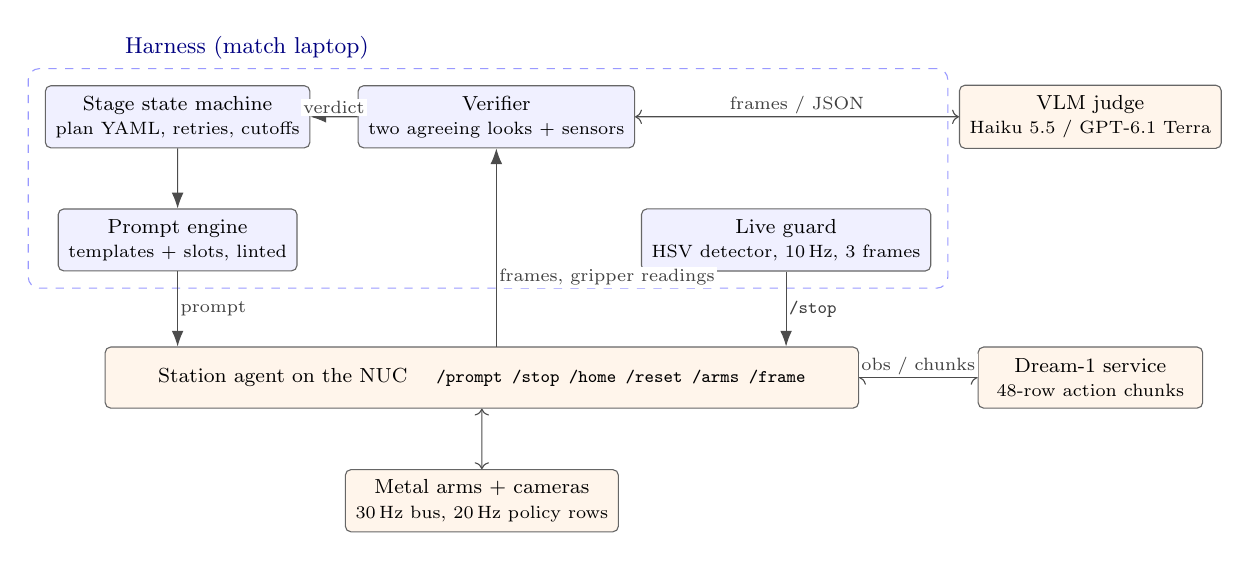
\begin{tikzpicture}[scale=0.92, transform shape,
  font=\footnotesize,
  box/.style={draw=black!60, rounded corners=2pt, align=center, minimum height=2.4em, inner sep=4pt, minimum width=31mm},
  hb/.style={box, fill=blue!6},
  ext/.style={box, fill=orange!8},
  arr/.style={-{Latex[length=2mm]}, black!70},
  lab/.style={font=\scriptsize, black!75, fill=white, inner sep=1pt}]
\node[hb] (sm)    at (0,3)   {Stage state machine\\ \scriptsize plan YAML, retries, cutoffs};
\node[hb] (pe)    at (0,1.3) {Prompt engine\\ \scriptsize templates + slots, linted};
\node[hb] (ver)   at (4.4,3) {Verifier\\ \scriptsize two agreeing looks + sensors};
\node[hb] (guard) at (8.4,1.3) {Live guard\\ \scriptsize HSV detector, 10\,Hz, 3 frames};
\node[ext] (judge) at (12.6,3) {VLM judge\\ \scriptsize Haiku 5.5 / GPT-6.1 Terra};
\node[ext, minimum width=104mm] (station) at (4.2,-0.6) {Station agent on the NUC \quad \scriptsize\texttt{/prompt /stop /home /reset /arms /frame}};
\node[ext] (dream) at (12.6,-0.6) {\dream{} service\\ \scriptsize 48-row action chunks};
\node[ext] (arms) at (4.2,-2.3) {Metal arms + cameras\\ \scriptsize 30\,Hz bus, 20\,Hz policy rows};
\node[draw=blue!40, dashed, rounded corners, fit=(sm)(pe)(ver)(guard), inner sep=6pt,
      label={[blue!50!black,font=\small]above left:{Harness (match laptop)}}] (h) {};
\draw[arr] (sm) -- (pe);
\draw[arr] (ver) -- node[lab, above]{verdict} (sm);
\draw[arr, <->] (ver) -- node[lab, above]{frames / JSON} (judge);
\draw[arr] (pe.south) -- node[lab, right]{prompt} (pe.south |- station.north);
\draw[arr] (ver.south |- station.north) -- node[lab, right, pos=0.35]{frames, gripper readings} (ver.south);
\draw[arr] (guard.south) -- node[lab, right]{\texttt{/stop}} (guard.south |- station.north);
\draw[arr, <->] (station.east) -- node[lab, above]{obs / chunks} (dream.west);
\draw[arr, <->] (station) -- (arms);
\end{tikzpicture}
\caption{The harness sits beside the station agent. It sends prompts and stop/home commands over local HTTP
and reads frames and gripper readings; every motor command, speed cap and clamp stays inside Dream's control
loop. The live guard has its own path to \texttt{/stop}, independent of the judge.}
\label{fig:arch}
\end{figure}

Figure~\ref{fig:arch} shows the structure. The harness runs on the match laptop, has no motor driver, and
talks only to the station agent. Preflight refuses to start if the station is busy, an arm is down, or a
camera frame is older than 2\,s. An arm fault, a station error, the time budget or an operator stop all send
\texttt{/stop}, which holds the arms where they are.

\subsection{Plans and the stage state machine}
A plan is a YAML list of stages. Each stage has a prompt (or a template), a yes/no success question, a
timeout, a retry budget, recovery prompts and an \texttt{on\_fail} policy. The top-level order follows the
rubric and the operator's notes: unplug every seated cable, optionally plug loose ones in, build the tower,
then balls. Because moving on from a pass-bar stage is a DQ, those stages retry until the clock runs out;
only scoring stages after a pass bar use the ``two tries, three if worth 20 points or more'' rule. Hard
cutoffs (for example, leave plug-in by $t=150$\,s) keep high-value but unreliable stages from starving later
ones. Retries use \texttt{/prompt} on the running session rather than stop and start, which costs 2.9\,s
(median) before motion resumes.

\subsection{Verification}
A stage is done only after two agreeing ``done'' verdicts. The judge receives a stitched grid: the stage-start
frame, the last six overhead frames and the newest wrist frames, with detector boxes drawn on them, and returns
JSON (\texttt{done}, \texttt{progress}, \texttt{status}, \texttt{holding}, \texttt{guard}). Two staggered calls
are kept in flight, which on the station halved the time between verdicts from about 9.7\,s to 4.9\,s.
Gripper readings from \texttt{/arms} overrule the judge's ``holding'' answer: a gripper closed fully on
nothing is not holding a cable, whatever the image seems to show.

\subsection{The live guard}
The illegal-ball guard cannot wait for a multi-second judge. A local detector (HSV thresholds, blob
extraction and a shape test that separates balls, cubes and lying sticks; no learned weights) runs on both wrist
frames at 10\,Hz in its own thread. Three consecutive positive frames send \texttt{/stop} directly, 0.3--0.5\,s
after the ball enters view. Detection on both wrist views takes 76\,ms per poll after vectorisation (236\,ms
before). The guard also blocks \texttt{/reset}, which moves both arms and cannot be cancelled once started.

\subsection{Prompting}
\label{sec:prompting}
Every instruction \dream{} receives comes from a template with slots (object colour, position, the next tower
piece, the current top piece), and no model writes free text to the robot. Templates are linted at load: a word
cap, no negations, no arm named in an arm-agnostic template, and no unfilled slot. Slots are filled from plan
defaults or by one cheap judge call that chooses among numbered options; a refill that produces the same text is
not resent. For a fine-tuned checkpoint the plan switches to \texttt{verbatim} mode, sending the recorded task
texts byte for byte, and the loader refuses any rewriting option alongside it.

These rules came from hand trials on the station with base \dream{} (Table~\ref{tab:prompts}). Three findings
shaped them. Naming an arm hurt: ``with the right arm'' forced the far arm onto blocks at the edge of its reach,
while the same request with no arm named was done by the left arm on the first try. Long, coached prompts did
worst; a 111-word cable prompt that described approach angle and cable orientation was the worst of the day.
And cable prompts are refused without a true safety sentence stating that the strip is unplugged and the cords
are insulated low-voltage USB. We stated the facts; we did not try to defeat the filter.

\begin{table}[t]
\centering
\small
\caption{Hand-tested prompts on the station (base \dream{}, 8 Nov). Counts are small and were judged by eye.}
\label{tab:prompts}
\begin{tabular}{@{}p{0.11\linewidth}p{0.55\linewidth}p{0.26\linewidth}@{}}
\toprule
Task & Prompt (abridged) & Outcome \\
\midrule
Unplug & ``With the right gripper half open, move down onto the plug \dots{} close the gripper on the plug and pull it straight up.'' + harness regrip and pull & held the plug through the pull, 2/2 \\
Unplug & ``Remove the first cable on the right from the power strip by pulling its plug straight up, then place it on the right side.'' & 1/3 (best policy-only wording) \\
Ball & ``With the right arm, pick up the orange golf ball on the right side of the table and drop it into the white basket.'' & in, $\sim$35\,s \\
Stack & ``put the pink cube on top of a blue cube'' (no arm named) & first try; repeat stacked the wrong cube \\
Stack & ``\dots{} lift it high and lower it gently straight down onto the blue cube, then open the gripper \dots'' & pink on blue, $\sim$85\,s \\
\midrule
Failed & arm named for stacking; whole-tower prompts; two arms in one prompt; ``eagle's-eye'' approach; direction words for pulling & see text \\
\bottomrule
\end{tabular}
\end{table}

\subsection{Harness-side skills and station tuning}
Two failure modes on the unplug resisted wording: \dream{} often closed the gripper on the way in, and it
pulled sideways so the plug came half out. We added two narrow skills that act only through the station's
existing move path. A \emph{regrip} opens the gripper to 0.6, lowers 1.5\,cm and closes when the gripper has
shut on nothing; a \emph{pull} lifts 6\,cm and then 4\,cm, 3\,s per step. An opt-in station add-on applies an
upward force of 20\,N while the right gripper holds. All station changes are opt-in environment variables,
refuse to load on any SDK other than the inspected version, and leave Dream's files unedited.

On a simulated Damiao bus running Dream's own driver, shortening the velocity feed-forward time constant from
0.8\,s to 0.15\,s cut joint tracking RMS by 40--50\%, while doubling the bus tick barely changed it
(Table~\ref{tab:tuning}). Requested 60\,Hz ticks reached 47--52\,Hz, because a late gripper reply holds each tick.

\begin{table}[t]
\centering
\small
\caption{Offline bench of Dream's Metal driver on a fake Damiao bus (0.4\,Hz sweep, gripper late half the
time). Tracking RMS per joint, degrees.}
\label{tab:tuning}
\begin{tabular}{@{}lcrrrrrr@{}}
\toprule
Setting & Bus tick (Hz) & j0 & j1 & j2 & j3 & j4 & j5 \\
\midrule
Stock: 30\,Hz, FF $\tau$ 0.8\,s & 30.0 & 2.24 & 2.89 & 3.64 & 4.46 & 1.73 & 1.74 \\
60\,Hz requested & 47--52 & 2.16 & 2.80 & 3.53 & 4.44 & 1.63 & 1.63 \\
30\,Hz, FF $\tau$ 0.15\,s & 29.8 & 1.37 & 1.73 & 2.19 & 2.31 & 1.18 & 1.19 \\
60\,Hz, FF $\tau$ 0.15\,s & 50.4 & \textbf{1.27} & \textbf{1.60} & \textbf{2.03} & \textbf{2.27} & \textbf{1.05} & \textbf{1.05} \\
\bottomrule
\end{tabular}
\end{table}

\subsection{Joint fault detection}
For monitoring the arms without brakes, we trained a per-joint fault detector on 16-reading windows (0.8\,s at
20\,Hz) of eight normalised features: position in range, margin to the nearer limit, velocity toward it, tracking
error, commanded velocity toward the limit, and measured, commanded and differential torque. Faults (limit run,
blocked joint, oscillation at 1.5--6\,Hz, overload, overspeed) and near misses were injected into 413k samples of
real policy motion from simulated matches, split by match file. Of 15 architectures, a dilated causal TCN~\cite{bai2018tcn}
(32 channels, 4 layers, 10.5k weights) had the best timely recall, $0.987\pm0.001$ over three seeds. On the held-out
file at a validation-chosen threshold it raised 0.2 false alarms per joint-hour at 0.91 timely recall, against 197
false alarms and 0.50 recall for the hand-written rules, whose limit-approach projection fires on every fast move
toward a limit. Overspeed bursts of 1--3 readings are the exception (0.68 vs.\ 0.93), so both run together. All
training motion is simulated YAM motion with injected faults; the numbers do not transfer to the Metal arms until it
is retrained on recorded CAN traces.

\section{A decision model for the harness}
\label{sec:decision}

The rules above are hand-set constants. To tune them we wrote them as a small model in which today's rules are a
special case. Let $x_t$ be the stage, the time in it, the time left $L$, the attempt count and the evidence features
$\phi(t)$ (judge verdict times confidence, judge progress, gripper transitions from \texttt{/arms}, detector boxes at
the goal, the hub's plug count from a cable-end classifier).

\paragraph{Done evidence.} A recursive log-odds score
\begin{equation}
  \ell_t = \gamma\,\ell_{t-1} + \textstyle\sum_i w_i\,\phi_i(t), \qquad \text{done} \iff \ell_t \ge \theta_{\text{done}}(s).
\end{equation}
The current rule (``two agreeing verdicts'') is $\gamma = 1$ on agreement and $0$ on disagreement, a single unit
weight on the judge, and $\theta_{\text{done}} = 2$.

\paragraph{The pass-bar constraint.} A false ``done'' on a pass bar leads the policy to touch the next stage's objects,
which is a DQ. If each look has false-positive rate $\alpha$ and $k$ independent looks are required,
$P(\text{false done}) \approx \alpha^k$, and $\theta_{\text{done}}$ is set per stage so that this stays under a budget
$\varepsilon$. Independence is the weak point. In the stress simulator, with two calls in flight, two false ``cable out''
verdicts arrived seconds apart and passed the two-look rule in 2 matches; the confirming looks shared the same frames.
A minimum gap between confirming verdicts would restore independence.

\paragraph{Fail hazard and action choice.} An attempt ends when
$h_t = \sigma\big(b + w_f n_{\text{fail}} + w_r[p_{\max}-p_t-\delta]_+ + w_s(\tau-\tau_{\text{rise}})/\tau_{\text{stall}} + w_T \tau/\tau_{\text{out}} - w_{\text{on}}\mathbb{1}[\text{on target}]\big)$
exceeds $\theta_{\text{fail}}$. The next action $a \in \{$continue, re-prompt, reset, home and retry, skip, abort$\}$ maximises
\begin{equation}
  Q(a\mid x) = P_a(\text{success within } c_a)\,V_s + W(L - c_a) - \lambda\,R_a,
\end{equation}
where $V_s$ is the stage's points plus the value it unlocks, $c_a$ the action's time cost, $R_a$ its DQ or illegal-ball
risk, and $W(L)$ the expected points of the remaining stages with $L$ seconds left, computed backwards over the plan from
each stage's success-versus-time curve $F_s(\tau)$. Continuing on stage $s$ is worthwhile while
\begin{equation}
  \frac{f_s(\tau)}{1-F_s(\tau)}\,V_s \;\ge\; \frac{dW}{dL},
\end{equation}
which gives each stage a timeout that depends on its own success hazard and on how much of the match remains.

\paragraph{Tuning objective.} $J(\theta) = \mathbb{E}[\text{points}] - \mu\,P(\text{DQ}) - \nu\,P(\text{illegal ball})$,
estimated in the stress simulator with common random numbers and searched by coordinate ascent or CMA-ES~\cite{hansen2016cma}.
A shadow-mode implementation logs what the model would do beside the live rules. We did not let it decide during the event,
and the noise model of the simulator still needs calibration from labelled station frames before its optimum can be trusted.

\section{Where the time goes}
\label{sec:latency}

\begin{figure}[t]
\centering
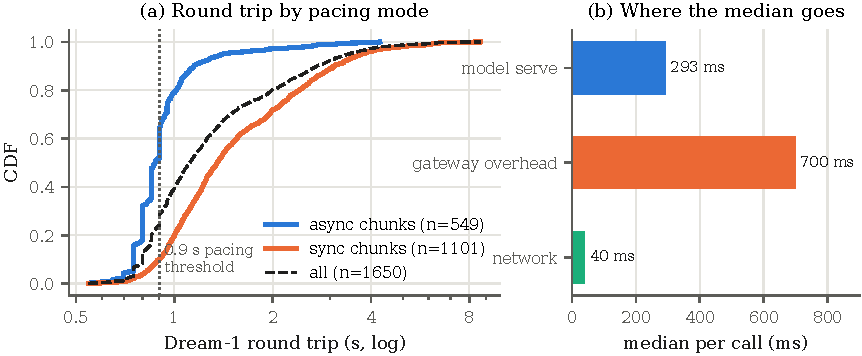
\includegraphics[width=\linewidth]{figs/latency.pdf}
\caption{\dream{} round trips on the station, 52 runs and 1{,}650 chunks between 18:06 on 7 Nov and 05:22 on 8 Nov
(UTC). (a) Chunks requested in stop-and-wait (sync) mode have the slow tail; the pacer switches mode around a 0.9\,s
median. (b) Median components as logged; medians are not additive, so the parts do not sum to the 1.12\,s median round trip.}
\label{fig:latency}
\end{figure}

The station logged every policy call (Figure~\ref{fig:latency}). The median round trip was 1{,}116\,ms (p10 800, p90
2{,}733, max 8{,}655). Of that, model serving took 293\,ms and the network 40\,ms; the rest is gateway overhead that we
cannot change. Each request uploads about 1.6\,MB of camera images, so a slow uplink adds directly: on a stretch at
8.8\,Mbit/s up, calls took 4.7\,s and the arm did nothing useful.

Because the median sits on the pacer's 900\,ms threshold, 67\% of chunks (1{,}101 of 1{,}650) ran stop-and-wait. In that
mode chunks arrive every 3.54\,s (median) for 2.4\,s of motion; in async mode every 1.55\,s with no gap. The arms
therefore stood still roughly 30\% of the time. Two things we controlled made it worse: the harness's own 2\,MB debug-view
fetches slowed calls to 2--6\,s until we switched to 35\,KB single frames, and fresh starts sometimes returned first
answers after 7--12\,s that the client discarded, costing about 20\,s per new session.

The harness adds its own delay at each stage boundary: a 3\,s poll, a judge call of several seconds, then a confirming
look. We estimate 5--8\,s of idle robot per boundary, or 25--40\,s of a 300\,s match. A local estimator that fuses gripper
and detector evidence (the $\ell_t$ above) could advance stages within about 0.5\,s and keep the judge as a parallel veto;
we designed but did not deploy it.

Errors were frequent enough to plan for. In the same window there were 16 policy errors: 4 safety refusals
(``unsafe instruction''; one triggered by a person's hand holding a plug), 4 \texttt{SVD did not converge} errors in the
client IK, 4 empty action buffers (12\,s without a chunk), and 4 replaced sessions. The harness now recovers from the
first three without ending the match: refusals retry with the template's safety sentence, and IK errors trigger at most
two automatic resets.

\section{Simulators}
\label{sec:sims}

\paragraph{Offline stress simulator.} The real \texttt{Runner} and judge client run unchanged; everything around them is
scripted. A virtual clock advances on every harness sleep, so a judge call returns only after its simulated latency and
races between checks, verdicts and the policy happen as they would live. A table model tracks cables, gripper contents,
the tower and the bin; each task prompt has a try time and a success probability, with switches for the failure modes we
saw (the policy will not release the plug, picks the illegal ball, brushes a block during the unplug, knocks the tower).
The station model injects faults with the exact error types and messages from the station log, plus frozen, empty, corrupt
and lagged camera frames and judge API outages. A scripted judge answers from the table state at the newest frame's
capture time. A referee scores rubric v4, including both DQ rules. A 5-minute match takes about 5\,s, so a 37-scenario
$\times$ 5-seed sweep fits on a laptop or our CPU cluster.

\paragraph{MuJoCo table with the real policy.} A drop-in replacement for the station agent serves the same HTTP routes on
Dream's MuJoCo YAM example~\cite{todorov2012mujoco}, with a relay table (hub, cables, blocks, golf balls, bin) laid out from
photographs and Dream's own control loop: camera windows, chunk requests to the live \dream{} API, chunk validation and
20\,Hz stepping. The harness cannot tell it from the station. The referee and an oracle verifier read object poses directly.
It ran in Docker on a four-node home cluster and on cloud batch VMs. Two caveats apply: the arm is a YAM, not a Metal arm,
so a Metal fine-tune cannot be evaluated here, and every match spends real policy credits.

\section{Results}
\label{sec:results}

\subsection{Harness robustness in the stress simulator}
Fixes made overnight turned faults that used to end a match into small losses (Table~\ref{tab:fixes}). The most
important was the plug: when the policy kept holding an unplugged plug, the old harness's next prompt led it to plug the
cable back in, which the rubric forbids, in 4 of 4 seeds. The fixed harness never did.

\begin{table}[t]
\centering
\small
\caption{Points per seed in the stress simulator before and after the robustness fixes (4 seeds).}
\label{tab:fixes}
\begin{tabular}{@{}lll@{}}
\toprule
Scenario & Before & After \\
\midrule
Happy path & 87, 74, 90, 116 & 83, 94, 95, 95 \\
Policy refuses on first start & 0, 0, 0, 0 (match ended) & 83, 94, 95, 95 \\
Empty action buffer mid-run & 10, 10, 15, 15 (ended) & 79, 94, 95, 100 \\
IK SVD failure & 10, 0, 10, 10 (ended) & 83, 84, 95, 95 \\
12\,s of corrupt frames & 20, 15, 20, 20 & 83--90 \\
Policy keeps the unplugged plug & plugged it back in, 4/4 & never \\
Illegal ball picked on 30\% of tries (6 seeds) & lost 4/6 & lost 2/6 (detector guard) \\
Unplug brushes a block & DQ 4/4 & DQ 4/4 \\
\bottomrule
\end{tabular}
\end{table}

\begin{figure}[t]
\centering
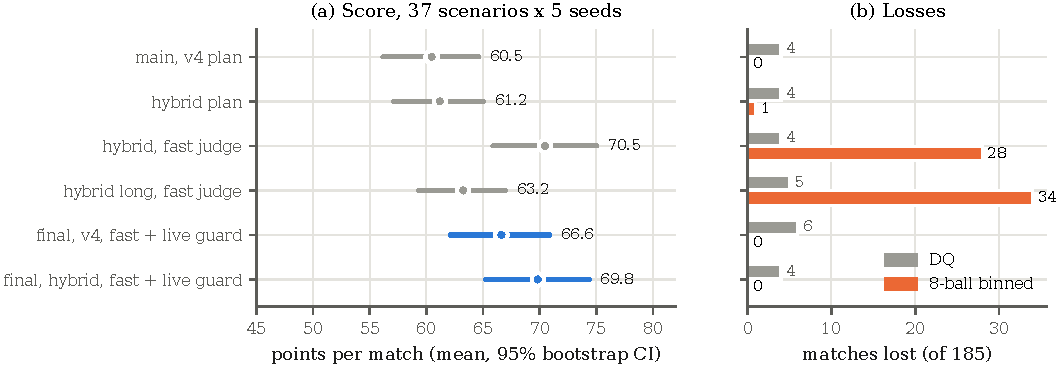
\includegraphics[width=\linewidth]{figs/stress.pdf}
\caption{Stress simulator, 185 matches per configuration (37 scenarios $\times$ 5 seeds). ``Fast'' judge: 4--6\,s per call;
otherwise 6.5--13\,s as measured for Haiku 5.5. Blue: configurations with the 10\,Hz live guard and gripper overrides.}
\label{fig:stress}
\end{figure}

Figure~\ref{fig:stress} compares whole configurations. Judge speed is the main lever on points, because a slow judge
rarely leaves time for the ball stage: at the measured latency, configurations binned 0 to 0.09 balls per match on average. But a fast judge
without the live guard reached the balls and lost 28 of 185 matches to the illegal ball (32 losses in total). With the guard
and sensor overrides, the hybrid plan kept 69.8 points (95\% CI 65.3--74.4) and lost none to the ball; the 4 remaining losses
are DQs from the \texttt{reach\_across} scenario, in which the policy brushes a block during the unplug, which no
supervisor can prevent after the fact. A longer plan with more cable stages scored lower and lost 34 matches to the ball.
Per-scenario means are in Appendix Figure~\ref{fig:scen}.

Two plan changes were selected by sweeping at the measured judge latency (24 scenarios $\times$ 4 seeds): removing
synchronous judge checks from stages that sensors can answer raised mean points from 54.9 to 60.0 with no new losses, and
dropping the extra cable stages from the base-model plan was worth about 18 points per match. Under scenarios calibrated to
base \dream{}'s observed unplug rate (about 1 try in 6), the plan written for the base model (colour and position prompts) beat the plan built on the fine-tune's recorded task texts by about 20 points.

These numbers test the harness's logic against a scripted world. The simulator's unplug probability of 0.8 per try is far
above what the real policy showed, and its judge never misjudges unless told to.

\subsection{Judges}
\label{sec:judges}

\begin{figure}[t]
\centering
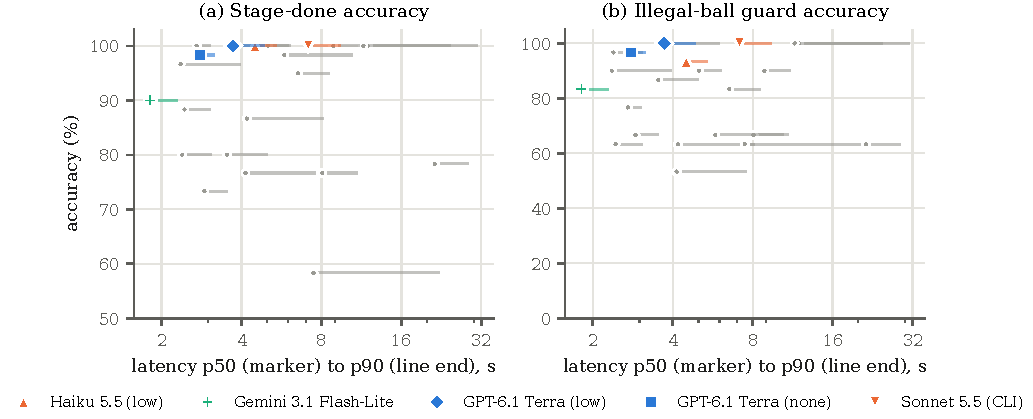
\includegraphics[width=\linewidth]{figs/judges.pdf}
\caption{Judge benchmark: 30 model and reasoning-level configurations, 60 decisions each (30 guard questions) on the
same frames, via OpenRouter or the Claude CLI. One configuration whose every call failed is omitted.}
\label{fig:judges}
\end{figure}

We benchmarked 30 judge configurations on the same 60 decisions (Figure~\ref{fig:judges}). Stage-done questions were easy
for most strong models; the guard question (``is a gripper holding the illegal ball?'') separated them. GPT-6.1 Terra with
no reasoning reached 98\% done and 97\% guard accuracy at a 2.8\,s median; with low reasoning, 100\% and 100\% at 3.7\,s, for
about \$0.07 per 60-decision match. Haiku 5.5 was perfect on done but 77--93\% on the guard depending on reasoning level;
Sonnet 5.5 through the CLI was perfect on both at 7.1\,s. On a separate 120-decision run, Haiku 5.5 caught a held illegal ball
only 55\% of the time. The guard result is the reason the live guard does not depend on any judge. With 30 guard questions per
configuration, a 100\% score has a 95\% lower bound of about 88\%, so these rankings are coarse.

\subsection{The real policy in MuJoCo}

\begin{table}[t]
\centering
\small
\caption{Base \dream{} through the harness on the MuJoCo relay table, 25 matches (one batch with a referee bug excluded).}
\label{tab:mujoco}
\begin{tabular}{@{}lll@{}}
\toprule
Task & Result & Time \\
\midrule
Unplug & a cable out in 14 of 25 matches & first unplug median 57\,s (28--269\,s) \\
Put the cable down & 0 of 54 tries & policy keeps holding the plug \\
Stack & 0 of 25 tries & -- \\
Balls & never reached & -- \\
DQs & 3, all with the hub on the left & -- \\
\bottomrule
\end{tabular}
\end{table}

Table~\ref{tab:mujoco} shows base \dream{} on the simulated table. It unplugged a cable in 14 of 25 matches, then kept
holding the plug and never put it down in 54 tries, so no match reached the tower. All 3 DQs occurred with the hub placed to
the left, where the plan's prompts (``the end of the hub nearest the right arm'') no longer matched the scene. Later batches put the
hub in front of the right arm, as on the station. In a separate 12-trial test, prompts naming an arm failed 0 of 4 times and the other arm
still moved for 10--19\,s; two goals in one prompt without naming arms completed one goal in 2 of 4 trials.

A cloud sweep meant to compare async pacing, operator notes and judge choice on this simulator (round~1, about 28 concurrent
policy sessions) stopped when the account's inference credits ran out. The service reported this as an unauthorised,
disabled key while account calls kept working. Only 10 of 28 matches were valid, scoring 0--42 points, and the comparison
cannot be made from them. We now probe the policy with one call before every batch.

\section{Teleoperation and fine-tuning}
\label{sec:teleop}

\subsection{Two collection paths on the Metal arms}
\paragraph{Leader/follower.} One Metal arm becomes the leader, running MakerMods' gravity-compensated leader mode
($k_p = 0$, Pinocchio~\cite{carpentier2019pinocchio} gravity and friction feed-forward); the other follows. We subclass the event
kit's collector so the dashboard, cameras, station lock, homing and LeRobot v2.1 writer are unchanged, and only the input differs.
The first real episodes showed the follower sitting below its command by gravity over $k_p$: shoulder lift $+4$ to $+6^\circ$,
elbow $+2.5$ to $+4.3^\circ$. Adding the leader's gravity model (which matches Dream's Metal gravity table to 0.01\,N\,m) to the
follower's MIT frames brought shoulder lift to $+0.2^\circ$.

\paragraph{Quest headset.} The kit's Quest path showed wrist flips: with joint 5 at its $-82^\circ$ limit margin, an 8--40$^\circ$
tool turn made the IK swing joints 4 and 6 by 130--190$^\circ$ over 1.5--2.5\,s. We added heading calibration, a One Euro
filter~\cite{casiez2012oneeuro} on controller poses, a wrist-flip guard that holds tool orientation when the wrist turns a lot for
little tool turn, a jump guard for tracking glitches, a 4\,rad/s wrist cap and gravity feed-forward. Replaying 40 fast-wrist events
from the recorded datasets through the IK, swings over $90^\circ$ fell from 7 of 40 (worst $194^\circ$) to 2 of 40 (worst
$116^\circ$) with tool position held within 8\,mm. On leader-recorded motion with Quest-like noise, wrist lag fell from 105\,ms to
27\,ms and median turn error from $2.8^\circ$ to $1.0^\circ$. These are offline replays; the new Quest launcher was not run with a
headset during the event.

\subsection{Why the fine-tune aimed high}
\label{sec:ft}

\begin{figure}[t]
\centering
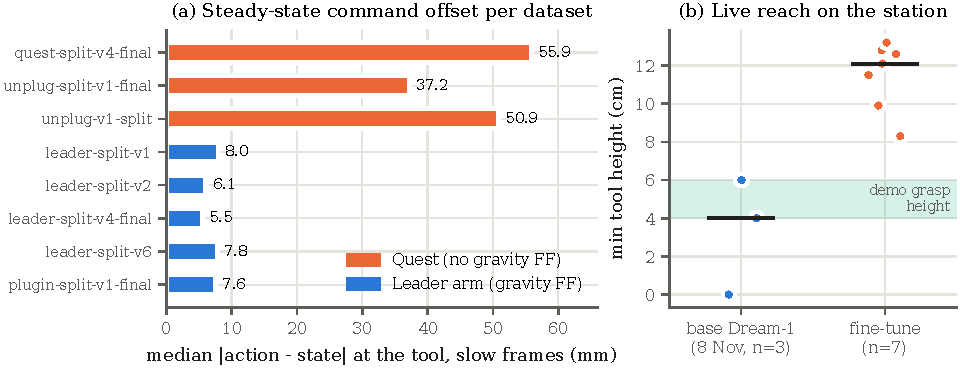
\includegraphics[width=\linewidth]{figs/finetune.pdf}
\caption{(a) Steady-state offset between commanded and measured tool position (frames with joint speed under 0.15\,rad/s, so lag
is excluded). Quest folders were recorded without gravity feed-forward. (b) Lowest tool height reached under the unplug prompt on the
station, base model vs.\ fine-tune; bars are medians. The fine-tune never reached the height at which demonstrations grasp.}
\label{fig:ft}
\end{figure}

The team fine-tuned \dream{} on 170 episodes (48{,}413 frames) from ten folders: 1{,}000 steps, learning rate $10^{-5}$, batch 32,
end-effector actions, constant schedule, final loss 0.0034. On the station it was worse than the base model on every task. Under the
unplug prompt its tool never went below 8--13\,cm while reaching, and it closed the gripper at 11--16\,cm; demonstrations grasp at
4--6\,cm, and the base model reached 0--6\,cm on the same day (Figure~\ref{fig:ft}b).

The cause is in the data (Figure~\ref{fig:ft}a). The 73 Quest episodes were recorded through the kit's follower, which sends zero
torque, so each joint sagged below its target. Their actions sit about 5.5\,cm (roughly $10^\circ$ across joints 2--4) above the
measured tool. The 97 leader episodes and the live station both apply gravity feed-forward, so command and arm agree to within
5--8\,mm. The model was trained on two incompatible maps from state to action: in Quest episodes, holding the tool at height $z$
takes a command at $z + 5.5$\,cm. Live, that command is reached, the arm rises, and it is asked to rise again. Unplug and put-down
are the tasks where both conventions appear (36 and 37 Quest episodes against 33 and 18 leader episodes).

We ruled out camera key mapping, view swaps, rotation, colour, resolution, camera position (under 2\,px shift), joint order and
units, gripper scaling, tool frame and schema differences across folders. Secondary causes were real but smaller: only 9 of 69
unplug demonstrations start within 0.3\,rad of the home pose every live run starts from; all four block demonstrations are
left-armed; playback at 20\,Hz against 30\,fps training adds about 80\,ms of lag, about 1\,cm at the arm's speeds.

To test whether a correction applied at run time could rescue the checkpoint, we built a MuJoCo model of one Metal arm with
Dream's link table, gains and feed-forward, fitted the effective gravity load to the Quest sag, and validated it (replaying Quest
actions without feed-forward reproduces recorded tool height with 10\,mm median RMS). Replaying the seven live fine-tune runs'
commands, no gravity scaling alone reached the 6\,cm grasp bar; the only correction that did without passing through the table was a
right-arm joint offset of 1.5 times the measured Quest sag, faded in with reach (grasp height 5.5\,cm, 1.8\,cm margin above the
table). This is an open-loop replay; the closed-loop policy would react to a lower arm. The data fix is simpler: replace each Quest
action with the measured joints three frames later before computing end-effector labels, and screen every folder for steady-state
action-minus-state offsets above about 1\,cm before training. A corrected 500-step fine-tune takes about five hours end to end, which
did not fit before the matches, so the final station plan ran base \dream{}.

\section{What we could not measure}
\label{sec:limits}

\begin{itemize}
  \item \textbf{No physical success rates.} The station log records calls and errors but not outcomes, and the harness logs that
  record per-stage outcomes were not collected from the station before the event ended. Table~\ref{tab:prompts} is judged by eye
  on a handful of trials. Human teleoperation times (unplug median 8.5\,s over 15 demonstrations; put-down 4.8\,s over 9) are the only
  real task timings we have.
  \item \textbf{Simulator fidelity.} The stress simulator's behaviour probabilities are assumptions, and its scenario mix is ours, so
  its absolute points are not predictions. The MuJoCo table uses a YAM arm, photo-estimated layout and an oracle verifier.
  \item \textbf{The real judge in the loop.} We benchmarked judges on fixed frames and ran the stress simulator with scripted verdicts,
  but did not run the real judge against the MuJoCo referee to measure false and late ``done'' rates.
  \item \textbf{Local detector colours} were tuned on phone photographs, not on station frames with a gripper closed around the white ball.
  \item \textbf{Fault detector} results are on simulated YAM motion with injected faults.
  \item \textbf{Tests.} The harness repository's last full run on its experimental branch was 407 passed, 4 failed, 5 skipped; two of the
  failures concern the async pacing test in the simulator.
\end{itemize}

\section{Lessons}

\begin{enumerate}
  \item \textbf{Under gating rules, the supervisor's false positives are the main risk.} A false ``done'' on a pass bar costs the whole
  match, so confirmation must use independent evidence: different frames, a minimum gap, or a different sensor.
  \item \textbf{Safety checks must not share a path with slow reasoning.} A 10\,Hz colour detector with its own \texttt{/stop} made a fast
  judge safe; no judge we tested was reliable enough on the guard question to stand alone.
  \item \textbf{Measure the serving loop before tuning prompts.} With a 0.9\,s pacing threshold and a 1.1\,s median round trip, request size
  and uplink decided whether the arms moved continuously. Our own debug traffic was part of the problem.
  \item \textbf{Prompt a VLA by naming objects, not arms or motions.} Colour and position helped; arm names, direction adverbs and long coaching
  hurt. Motions the words could not fix (regrip, pull) were better done as small, separately tested skills.
  \item \textbf{Check action-minus-state per data source before fine-tuning.} Two collection paths on the same arm differed by 5.5\,cm in
  steady state, and the training loss gave no sign of it.
  \item \textbf{Log outcomes, not just calls.} Without per-stage outcome logs on the station, a night of runs produced latency statistics
  but no success rate.
\end{enumerate}

\section{Conclusion}
For a hosted VLA under a strict rubric, most of the engineering we could do sat outside the policy: when to declare a stage done,
how fast to stop, what words to send, how to keep the serving loop in async mode, and whether the demonstration data agreed with
the robot's control path. The harness, both simulators, the teleoperation tools and the analysis scripts are public. The next
experiments are the ones the event did not leave time for: per-stage outcome logging on the station, the real judge against the
MuJoCo referee, and a fine-tune on gravity-corrected data compared with the base model on the same seeded scenes.

\section*{Acknowledgments}
We thank MakerMods and Dream Labs for the stations, \dream{} access and the event kit, and Founders Inc for hosting Physical AI Hacks.
Much of the code and analysis was written with AI coding assistants (Anthropic's Claude Code and OpenAI's Codex) under the authors'
direction; the authors chose the experiments, ran the station, and checked the results reported here.

\bibliographystyle{unsrtnat}
\bibliography{refs}

\appendix
\section{Per-scenario results}

\begin{figure}[h]
\centering
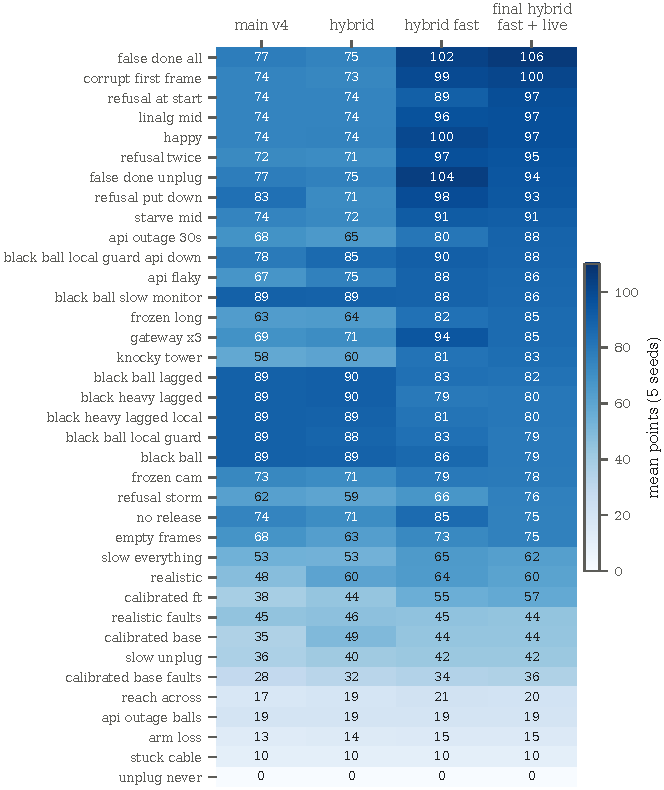
\includegraphics[height=0.62\textheight]{figs/scenarios.pdf}
\caption{Mean points per stress scenario (5 seeds each), sorted by the final configuration. Scenarios include API outages, refusals,
frozen and corrupt cameras, false ``done'' verdicts, an illegal ball near the bin, a knock-prone tower, and \texttt{unplug\_never}, in
which no configuration can score.}
\label{fig:scen}
\end{figure}

\section{Reproducing the numbers}
\begin{sloppypar}
\begin{itemize}
  \item Stress sweep: \texttt{cluster/run\_stress.sh 50 7 sweep1}, aggregated by \texttt{results/stress/final\_20261108/analyze.py}
  in \texttt{task\_simulation}.
  \item MuJoCo matches: \texttt{python sim\_station.py --policy dream --scene hill\_climb} with \texttt{experiments/sim\_match.py}, or
  \texttt{cluster/run\_matches.sh}; requires a \dream{} key with credit.
  \item Station latency, stress and judge figures: \texttt{paper/make\_figures.py} reads the logged files listed in its header.
  \item Quest replay bench: \texttt{quest/bench} in \texttt{follower\_code} (branch \texttt{quest-continuity}).
\end{itemize}
\end{sloppypar}

\end{document}
